\section{Introduction}
\begin{frame}{Plasma}
  \begin{itemize}
    \item Plasma is an ionized gas that consists of highly energized particles, including positively charged ions and negatively charged electrons.
  \end{itemize}

  \begin{figure}[htbp]
    \centering
    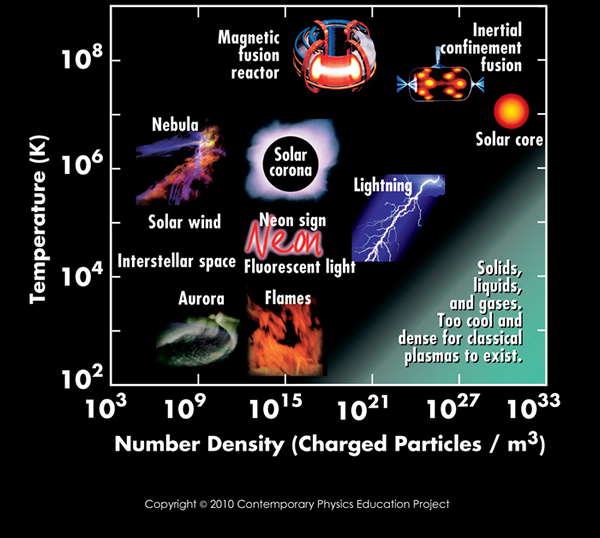
\includegraphics[width=0.5\textwidth]{../../thesis/img/introduction/plasma-properties}
    \caption{Characteristics of typical plasmas.}
    \label{fig:plasma-properties}
  \end{figure}
\end{frame}

\begin{frame}{Magnetic Nozzle}
  \begin{itemize}
    \item A magnetic nozzle is a device that uses a magnetic field to shape and control the flow of charged particles in a plasma propulsion system.
  \end{itemize}
\begin{figure}[htbp]
  \centering
  \begin{subfigure}{0.45\textwidth}
    \centering
    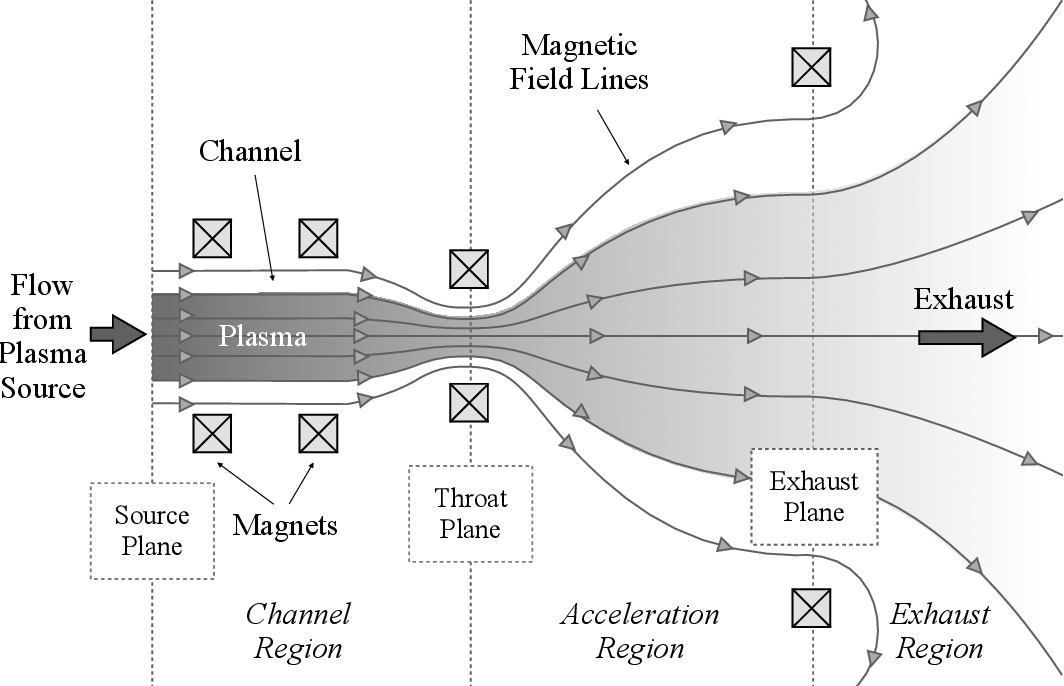
\includegraphics[width=\linewidth]{../../thesis/img/introduction/magnetic-nozzle}
    \caption{Simplified representation of magnetic nozzle.} 
  \end{subfigure}%
  \begin{subfigure}{0.45\textwidth}
    \centering
    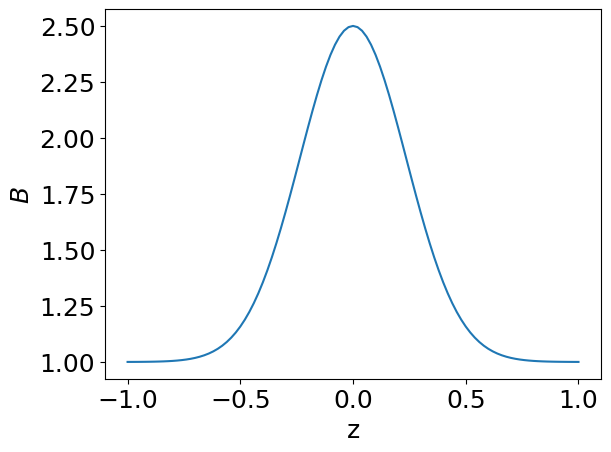
\includegraphics[width=\linewidth]{../../thesis/img/introduction/magnetic-field.png}
    \caption{A simplified magnetic field of magnetic nozzle.} 
  \end{subfigure}
  \caption{The length of the magnetic nozzle is normalized, so it is extended from -1 to 1.}
	\label{fig:magnetic-nozzle}
\end{figure}
\end{frame}

\begin{frame}{Instability of Plasma Flow}
  \begin{itemize}
    \item The instability of plasma flow refers to the tendency of a plasma system to deviate from a stable, equilibrium state and exhibit perturbations or fluctuations in its behavior.
    \item Plasma instabilities plays a significant role in the transport of energy.
  \end{itemize}  
\end{frame}

\begin{frame}{Significance of this research}
  The importance of this research is listed below:
  \begin{itemize}
    \item One configuration in magnetic nozzle is so-called magnetic mirror.
    \item Examples having magnetic mirror configuration: Bondi-Parker flow, convertor-divertor in linear fusion device. \cite{bondi_spherically_1952,aikawa_stability_1979,keto_stability_2020,smolyakov_quasineutral_2021}
  \end{itemize}
\end{frame}

\begin{frame}{Goals of this thesis}
  \begin{itemize}
    \item Understand the standard technique to tackle instability problems.
    \item Understand and apply spectral method to our problem.
    \item Investigate the instability of the plasma flow with different velocity profile in magnetic nozzle under different boundary conditions.
    \item Investigate the effects of the presence of singularity in transonic velocity profile.
  \end{itemize}  
\end{frame}
